\begin{itemize}
\item A relation $R$ on a set $A$ is an equivalence relation if it is 
reflexive, symmetric, and transitive.
\item When the elements of some set $A$ have a notion of equivalence defined on 
them, then one may naturally split the set $A$ into equivalence classes.
\item If $R$ is an equivalence relation on the set $A$, its equivalence classes 
form a partition of $A$.
\item In each equivalence class, all the elements are related and every element 
in $A$ belongs to one and only one equivalence class.
\item The relation $R$ determines the membership in each equivalence class, and 
every element in the equivalence class can be used to represent that equivalence 
class.
\item In a sense, if you know one member within an equivalence class, you also 
know all the other elements in the equivalence class because they are all 
related according to $R$.
\item Conversely, given a partition of $A$, we can use it to define 
an equivalence relation by declaring two elements to be related if they belong 
to the same component in the partition.
\end{itemize}
\begin{figure}[H]
\centering
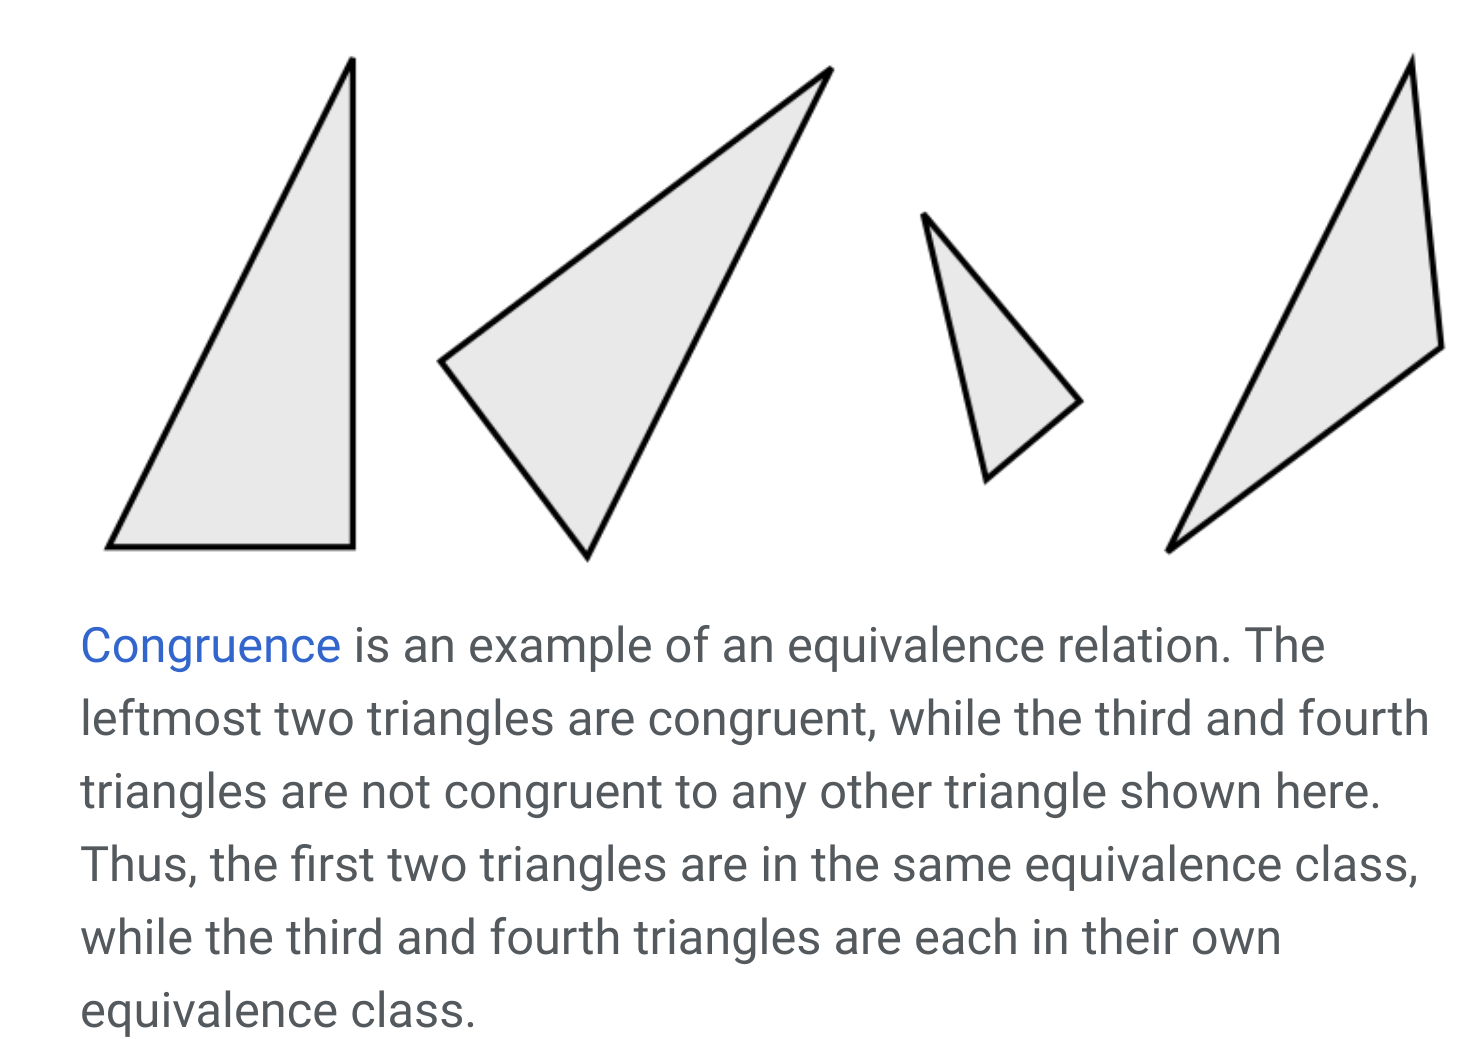
\includegraphics[width=0.5\textwidth]{equ-class.png}
\end{figure}
Ref: 
\begin{itemize}
\item \href{
https://math.libretexts.org/Courses/Monroe_Community_College/MTH_220_Discrete_Ma
th/6\%3A_Relations/6.3\%3A_Equivalence_Relations_and_Partitions}{equivalence}
\item \href{https://en.wikipedia.org/wiki/Equivalence_class}{Equivalence Class}
\end{itemize}